\documentclass[onehalf,11pt]{beavtex}
\title{Type-Safe Sandboxing of Memory-Unsafe C/C++ Libraries for Rust Programs}
\author{Jonathan Keller}
\degree{Master of Science}
\doctype{Thesis}
\department{Electrical Engineering and Computer Science}
\depttype{School}
\depthead{Head}
\major{Computer Science}
\advisor{Yeongjin Jang}
\coadvisor{Yeongjin Jang}
\submitdate{May 20, 2024}
\commencementyear{2024}
\abstract{
    As the software engineering industry adopts memory-safe programming languages for security- and
    performance-sensitive systems programming, developers face a need for interoperability between
    memory-safe and memory-unsafe codebases, without compromising on either security or performance.
    We present a technique for sandboxing unsafe dependencies within a safe program, using hardware
    features such as Intel's Memory Protection Keys to prevent memory corruption bugs within unsafe
    code from affecting the safe portions of the program. We use the type system and metaprogramming
    capabilities of the Rust programming language to create a low-overhead, ergonomic, and type- and
    memory-safe interface allowing the safe portions of the program to freely interact with the
    unsafe portions, without risk of inducing undefined behavior in memory-safe code.
}


% \usepackage{algorithm}
% \usepackage{algorithmic}

% common packages
\usepackage{silence}
\WarningFilter*{caption}{Unsupported document class}

\usepackage[hyphens]{url}
\usepackage[breaklinks,colorlinks]{hyperref}
\usepackage[usenames,dvipsnames]{xcolor}
\hypersetup{citecolor=blue,linkcolor=blue}
\usepackage{amsmath,amsopn,amssymb}
\usepackage{subcaption}
\usepackage{endnotes,microtype,xspace,graphicx,fancyvrb,multirow}
\usepackage{booktabs}
\usepackage{array,underscore,relsize}
\usepackage[T1]{fontenc}
\usepackage{times}
\usepackage{fancyhdr,lastpage}
\usepackage{enumitem}
\usepackage[labelfont=bf,font=small,skip=5pt]{caption}
\pagestyle{fancy}
\fancyhf{}
\renewcommand{\headrulewidth}{0pt}
\cfoot{\thepage}

% for math macro and numbers
\usepackage{fp}
\usepackage{siunitx}

% pseudo code
\usepackage{minted}

% balance bibliography
\usepackage{balance}

% use \num{123456} -> 123,456
\sisetup{group-separator={,},group-minimum-digits={3},output-decimal-marker={.}}


\newcommand{\sys}{\mbox{\textsc{Die}}\xspace}

% ref. http://en.wikibooks.org/wiki/LaTeX/Colors
\newcommand{\YJ}[1]{\textcolor{blue}{MK: #1}}
\newcommand{\JK}[1]{\textcolor{orange}{SK: #1}}
\newcommand{\XX}[0]{\textcolor{red}{XXX}}
\newcommand{\XXX}[1]{\textcolor{red}{XXX: #1}}
\newcommand{\TODO}[1]{\textcolor{Melon}{TODO: #1}}

\newcounter{definition}
\newcommand\definitionautorefname{Definition}
\DeclareCaptionType{definition}
%\newfloat{definition}{htbp}{.nb}

\renewcommand{\ttdefault}{pxtt}

\newcommand{\URL}{\url}
\newcommand{\cc}[1]{\mbox{\smaller[0.5]\texttt{#1}}}

% enable the below for ACM camera ready
%\clubpenalty=10000
%\widowpenalty=10000
%\renewcommand*{\bibfont}{\raggedright}

%\linespread{1.2}

\fvset{fontsize=\scriptsize,xleftmargin=8pt,numbers=left,numbersep=5pt}

\input{code/fmt}
\newcommand{\figrule}{\hrule width \hsize height .33pt}
\newcommand{\coderule}{\vspace{-0.5em}\figrule\vspace{0.2em}}

\setlength{\abovedisplayskip}{0pt}
\setlength{\abovedisplayshortskip}{0pt}
\setlength{\belowdisplayskip}{0pt}
\setlength{\belowdisplayshortskip}{0pt}
\setlength{\jot}{0pt}

\def\Snospace~{\S{}}
\renewcommand*\sectionautorefname{\Snospace}
\def\sectionautorefname{\Snospace}
\def\subsectionautorefname{\Snospace}
\def\subsubsectionautorefname{\Snospace}
\def\chapterautorefname{\Snospace}
%\renewcommand{\figurename}{Fig.}
%\def\figureautorefname{\figurename}
%\newcommand{\subfigureautorefname}{\figureautorefname}

%\numberwithin{equation}{section}
\newcommand{\yes}{Y}
\newcommand{\no}{}

% sema
\newcommand{\shl}{\ \cc{<}\cc{<}\ }
\newcommand{\shr}{\ \cc{>}\cc{>}\ }
\newcommand{\x}{$\times$\xspace}

\if 0
\renewcommand{\topfraction}{0.9}
\renewcommand{\dbltopfraction}{0.9}
\renewcommand{\bottomfraction}{0.8}
\renewcommand{\textfraction}{0.05}
\renewcommand{\floatpagefraction}{0.9}
\renewcommand{\dblfloatpagefraction}{0.9}
\setcounter{topnumber}{10}
\setcounter{bottomnumber}{10}
\setcounter{totalnumber}{10}
\setcounter{dbltopnumber}{10}
\fi

\newif\ifdraft\drafttrue
\newif\ifnotes\notestrue
\ifdraft\else\notesfalse\fi

% hide comments
% \renewcommand{\TK}[1]{\ignorespaces}
% \renewcommand{\XXX}[1]{\ignorespaces}
% \renewcommand{\TODO}[1]{\ignorespaces}

%% Ensure ligatures (e.g., ``fine official flag'') can be copy/pasted from PDF.
\input{glyphtounicode}
\pdfgentounicode=1

\newcolumntype{R}[1]{>{\raggedleft\let\newline\\\arraybackslash\hspace{0pt}}p{#1}}

% include macros
\newcommand{\includepdf}[1]{
  \includegraphics[width=\columnwidth]{#1}
}
\newcommand{\includeplot}[1]{
  \resizebox{\columnwidth}{!}{\input{#1}}
}

% list
\newcommand{\squishlist}{
\begin{itemize}[noitemsep,nolistsep]
  \setlength{\itemsep}{-0pt}
}
\newcommand{\squishend}{
  \end{itemize}
}

%%
%% NOTE.
%%  to use circled number in caption, use
%%   (e.g., \protect\WC{1})
%%
\usepackage{tikz}
\newcommand*\WC[1]{%
\begin{tikzpicture}[baseline=(C.base)]
\node[draw,circle,inner sep=0.2pt](C) {#1};
\end{tikzpicture}}

\newcommand*\BC[1]{%
\begin{tikzpicture}[baseline=(C.base)]
\node[draw,circle,fill=black,inner sep=0.2pt](C) {\textcolor{white}{#1}};
\end{tikzpicture}}

\usepackage{xstring}
\newcommand{\PP}[1]{
\vspace{2px}
\noindent{\bf \IfEndWith{#1}{.}{#1}{#1.}}
}

\newcommand{\PN}[1]{
\vspace{2px}
\noindent{\bf #1}
}

\newcommand{\ra}[1]{\renewcommand{\arraystretch}{#1}}
\newcommand{\V}{\checkmark}
\newcommand{\X}{{\footnotesize $\times$}\xspace}
\renewcommand{\O}{\phantom{0}}

%% units
\newcommand{\B}{\,\text{B}\xspace}
\newcommand{\K}{\,\text{K}\xspace}
\newcommand{\M}{\,\text{M}\xspace}
\newcommand{\T}{\,\text{T}\xspace}
\newcommand{\KB}{\,\text{KB}\xspace}
\newcommand{\MB}{\,\text{MB}\xspace}
\newcommand{\GB}{\,\text{GB}\xspace}
\newcommand{\TB}{\,\text{TB}\xspace}

\newcommand{\Bs}{\,\text{B/s}\xspace}
\newcommand{\KBs}{\,\text{KB/s}\xspace}
\newcommand{\MBs}{\,\text{MB/s}\xspace}
\newcommand{\GBs}{\,\text{GB/s}\xspace}

% boxbeg/end
\newcommand{\boxbeg}{
\vspace{2px}
\noindent\begin{tabular}{|l|}\hline
\begin{minipage}{3.2in}
\vspace{2px}
\noindent
}

\newcommand{\boxend}{
\vspace{2px}
\end{minipage}\\ \hline
\end{tabular}
\vspace{-10pt}
}

\input{rev}

\begin{document}
\maketitle

\mainmatter

\chapter{Introduction}

In recent years the systems programming industry has seen increased adoption of memory-safe
programming languages such as Rust, due to their ability to categorically prevent memory corruption
bugs and the associated security risks. However, in a mixed program containing both memory-safe and
memory-unsafe code within the same address space, memory corruption issues in the memory-unsafe
portions can still lead to manipulation or takeover of the entire program, as the properties of
memory safety do not restrict or limit undefined behavior caused by memory-unsafe
code~\cite{hu:crust, lolcads:e2va}; this class of vulnerability is listed in MITRE's Common Weakness
Enumeration database as CWE-111~\cite{mitre:cwe-111}.

Ideally, modern software systems would be designed from the ground up in memory-safe programming
languages (such as Java, Python, or Rust), but this is often infeasible in practice due to the costs
of rewriting large amounts of legacy code. Thus, many real-world software systems combine
memory-safe and memory-unsafe code within the same program, such as by adding memory-safe components
to a mostly memory-unsafe codebase, or by embedding memory-unsafe libraries into memory-safe
applications~\cite{rust:ffi, oracle:jni}. Such a mixed program has a smaller attack surface than one
written entirely in a memory-unsafe language, but the memory-unsafe components still present an
attractive exploitation target, as an attacker who exploits a vulnerability such as a buffer
overflow or use-after-free in memory-unsafe code may be able to corrupt variables used by
memory-safe portions of the program.

Software fault isolation is a family of techniques that can be used to separate a program into
protection domains and achieve memory protection between domains~\cite{wahbe:sfi}. Within the
context of a program containing a mixture of memory-safe and memory-unsafe code, software fault
isolation can be used to prevent vulnerabilities within memory-unsafe code from affecting the
integrity of data used by safe code. There is existing research demonstrating the application of
software fault isolation to this problem space~\cite{ghoshn:enclosure, kirth:pkru}, but even with
such protection the authors of the memory-safe portions of such a program must take caution when
accessing values produced by memory-unsafe code, as memory corruption within memory-unsafe code may
result in invalid values that violate invariants expected by the memory-safe programming language.
For example, if the memory-safe portion of the program dereferences a pointer produced within the
memory-unsafe portion without proper validation, an attacker may be able to corrupt the address of
the pointer in a way that causes the memory-safe code to corrupt its own memory.

We present a scheme for automatically sandboxing memory-unsafe C code within a Rust program, using
x86 Memory Protection Keys (MPK)~\cite{intel:system, linux:mpk} to maintain separation between data
used by the memory-unsafe and memory-safe portions of the program. MPK allows the kernel to tag page
table entries with protection keys, and allows user programs to dynamically restrict access to
memory tagged with specific keys without the need for a system call. We use this capability to limit
the ability of memory-unsafe code to access memory belonging to the safe portions of a program,
maintaining the integrity of the memory-safe portions of the program even if the attacker can
corrupt the memory-unsafe portions.

We modified Rust's \cc{bindgen} library to generate safe interfaces to sandboxed code.
\cc{bindgen}~\cite{rust:bindgen} is a procedural macro that generates Rust interfaces to code
written in other programming languages such as C and C++; we modified \cc{bindgen} to automatically
manage the process of configuring MPK while entering and exiting the sandbox. Additionally, we
define a type-safe interface allowing an application to interact with pointers and data accessible
to sandboxed code without risk of misuse leading to undefined behavior. We achieve this using a
combination of compile-time invariants expressed using Rust's type system and borrow checker, and
low-cost runtime checks verifying pointer bounds and alignment.

We measured a performance overhead of approximately 25ns each time a function call and return
crosses the boundary between protected and sandboxed code. The impact of this on a production
application will vary depending on how many function calls the application makes relative to the
work performed within the sandboxed function; we measured a 7\% performance overhead in a benchmark
that uses the \cc{cmark} Markdown parsing library to parse a small document within a sandbox, and a
negligible overhead in a benchmark that invokes sandboxed \cc{cmark} on a larger document.

Our work shows that MPK can application programs today can benefit from lightweight, low-overhead,
secure sandboxing as a simple line of defense against supply-chain attacks through memory-unsafe
code. Our implementation does not completely eliminate memory corruption as an attack vector, it
only limits the scope of data that an attacker can corrupt. Additionally, it it is not completely
transparent: the Rust programmer must make small modifications to the portions of their program that
interact with memory-unsafe code. However, our work towards automatically generating safe interfaces
to sandboxed code greatly reduces the development effort and likelihood of making security-critical
mistakes compared to approaches that require the programmer to directly interact with unsafe
functions. And as our sandboxing scheme requires no compiler modifications or language extensions,
it is simpler to integrate into real-world applications than schemes that require large amounts of
custom compiler tooling or break compatibility with existing applications.

\paragraph{Source Code} Our code is available on GitHub at
\url{https://github.com/NobodyNada/thesis}.

\chapter{Background}

In this section, we provide some context on memory corruption issues and techniques used to mitigate
them, such as memory-safe programming languages and memory sandboxing techniques.

\section{Memory Safety}

\paragraph{Memory Corruption} Memory-corrupting software bugs are the leading cause of exploitable
security vulnerabilities in computer programs -- recent analysis on large, industry-leading software
projects has consistently shown that between 60-90\% of high-severity vulnerabilities are caused by
memory corruption~\cite{google:android-vulns, google:android-vulns-2, chromium:memory-safety,
msrc:memory-safety}. Memory corruption occurs when a program, due to improper input validation or
developer oversight, mistakenly reads or writes to an incorrect location in memory. Memory
corruption can have a variety of effects depending on what memory was mistakenly accessed, including
causing the program to crash, exposing sensitive information, corrupting variables or data
structures used elsewhere in the program, or altering the control flow of a program.
Memory-corrupting bugs are common due to the complexity and difficulty of memory management, and
they are a dangerous tool in the hands of an attacker due to their wide-ranging effects.

Memory-corruption bugs can be broadly divided into two categories: \textit{spatial} and
\textit{temporal} memory corruption.

\squishlist
    \item Spatial memory corruption is caused by a program accessing an incorrect location in memory
        -- for example, a buffer overflow is a type of spatial memory issue caused by reading or
        writing past the end of an object in memory.
    \item Temporal memory corruption is caused by a program accessing a location in memory that used
        to be valid but is no longer so. For example, a use-after-free is a type of temporal memory
        issue caused when one part of a program deallocates (and possibly reallocates for another
        purpose) memory that is still in use elsewhere in the program.
\squishend

Semantically, memory-corruption bugs are considered a type of \textit{undefined behavior}: due to
the unpredictable and severe effects of memory corruption, a programming language specification will
typically not make guarantees of the behavior of a program that corrupts memory. In other words:
anything can happen in the presence of memory corruption, including malfunctions or further memory
corruption in seemingly unrelated parts of the program.

\paragraph{Memory Safety} A \textit{memory-safe} programming language is one where programs
exhibiting spatial or temporal memory corruption are not representable in the semantics of the
language. Spatial memory corruption is relatively straightforward to prevent at the language level
by designing a language to include bounds information within dynamically-sized objects (such as
arrays and strings), checking all accesses to such objects at runtime, and aborting with an error if
the access would exceed the bounds of the object. Although there is a theoretical performance
overhead to the additional bounds checks, in practice the overhead is typically negligible with a
modern optimizing compiler and superscalar CPU. Temporal memory safety is harder to achieve, as it
requires the language implementation to perform some form of liveness analysis to determine when it
is safe to deallocate memory.

Historically, most memory-safe languages (such as Java or Python) have achieved memory safety by
limiting the programmer's ability to access memory, exposing only high-level object-oriented
abstractions rather than giving direct control over memory usage and allocation. These languages
typically include managed runtimes which track object lifetimes using garbage collection techniques
such as tracing or reference counting, which involve maintaining records of memory reachability at
runtime in order to determine when a region of memory is no longer in use. However, the performance
and memory overhead of dynamically tracking memory reachability is not negligible, and the lack of
direct control over managed memory prevents programmers from being able to express many important
design patterns, optimizations, and hardware interfaces. For this reason, memory-safe languages have
typically been considered unsuitable for performance-sensitive systems programming.

\paragraph{Rust} Rust~\cite{rust} is a relatively new memory-safe programming language designed for systems
programming. In order to achieve memory safety without compromising performance, it has a complex
type system that statically tracks the lifetimes of objects. The Rust compiler includes a
\textit{borrow checker} that uses this type information to validate the lifetimes of all objects in
memory at compile time, ensuring all temporal memory safety issues raise a compile-time error,
without adding any runtime overhead to the compiled program.

\paragraph{Reference Types} To express pointer semantics in a memory-safe and statically verifiable
manner, Rust introduces a checked reference type, spelled \cc{\&T} (for an immutable reference to an
object of type \cc{T}) or \cc{\&mut T} (for a mutable reference.) A reference type has a
\textit{lifetime} associated with it, indicating a duration for which the reference is guaranteed to
point to a valid object. Creating a reference involves \textit{borrowing} an owned object, and the
lifetime of the borrowed reference lasts no longer than the program scope of the referenced object.
Additionally, the borrow checker enforces aliasing rules that prevent concurrent modification of
referenced data in order to prevent bugs caused by two references unexpectedly pointing to the same
object.

Not all memory usage patterns can be represented in Rust's type system, and so the language includes
an \cc{unsafe} keyword that can be used to perform operations that may be memory-unsafe, including
accessing memory without bounds or lifetime checks, so that programmers can implement patterns that
are desirable for performance or compatibility reasons but are impossible in safe Rust. Rust
developers are encouraged to create safe abstractions around unsafe patterns, by using Rust's type
system to design APIs that provide a safe interface to unsafe code.

In recent years, the prevalence of security issues caused by memory corruption issues has prompted
the industry to move towards memory-safe languages such as Rust. Companies such as
Google~\cite{google:android-rust} and Microsoft~\cite{msrc:memory-safety} have been increasingly
adopting memory-safe programming languages in order to improve security, and recently the United
States Cybersecurity and Infrastructure Security Agency, together with a number of US and
international security agencies, released a report advocating for a transition to memory-safe
programming languages~\cite{cisa:memory-safety}.

\section{Software Dependencies and Supply-Chain Security}

Modern software is rarely written from scratch. Most programs depend on many third-party libraries
to implement common functionality -- and even if a program is written in a memory-safe language, it
may need functionality from a library written in a memory-unsafe language. Additionally, if someone
wishes to migrate memory-unsafe software to a memory-safe language, they may choose to do so
incrementally or partially, resulting in a program containing a mix of memory-safe and memory-unsafe
code.

\paragraph{Partial Memory-Safety} While a partially memory-safe program is more secure than an
entirely memory-unsafe program, there are still significant risks when combining memory-unsafe and
memory-safe code. Vulnerabilities in the memory-unsafe parts of the program are still exploitable,
and memory corruption in memory-unsafe code can induce undefined behavior and further memory
corruption in memory-safe code. In fact, memory corruption in a mixed program may under some
circumstances be \textit{more} severe than in a purely memory unsafe program because the memory-safe
portions of the code may elide runtime safety checks due to the guarantees provided by memory-safe
code. Additionally, it is often difficult to reason about the correctness of a program at the
boundaries between memory-safe and memory-unsafe code because of inter-language differences in
guarantees and requirements regarding memory layout and lifetimes.

Our work focuses specifically on interaction between Rust and C/C++, but this problem affects any
situation where memory-safe code is interacting with memory-unsafe code in the same process, such as
the Java Native Interface, or Python libraries that call out to C/C++ code. Our methods will be
largely generalizable to other languages as well, though the specific implementations may differ to
meet different languages' precise semantics around memory safety.

\paragraph{Supply-Chain Vulnerabilities} The use of third-party dependencies in a program introduces
a risk of exposure to supply-chain security vulnerabilities: when a vulnerability is discovered in a
commonly-used library, all applications using the library are potentially at risk of exploit. And
while many security vulnerabilities in libraries only apply to applications using the library in
specific ways and/or limit the capabilities of the attacker to the capabilities of the library
within the larger application, memory corruption in a third-party library can often lead to total
compromise of dependent applications because of the ability of memory corruption to affect unrelated
parts of the program. As a particularly recent example, the recently-discovered backdoor in the
widely used \cc{xz} data compression library demonstrates how an entire application can be
compromised by a seemingly insignificant third-party dependency.

Due to its wide use and high risk, we identified interoperability between memory-unsafe and safe
code as an important target for research, and searched for ways to limit the security impact of
memory corruption in mixed codebases.

\section{Sandboxing and Software Fault Isolation}

A defense-in-depth approach to software security involves not just designing software to be free of
vulnerabilities (for instance, by using memory-safe languages), but also taking steps to mitigate
the impact of vulnerabilities when they do arise. Software sandboxing is the practice of limiting
the capabilities granted to part of a program so that an attacker who gains control over that part
of the program has only limited control over the entire system. For example, web browsers typically
render each web page the user is visiting within a separate process, so that an attacker who is able
to exploit a bug in the high-complexity, high-risk rendering engine is unable to control or extract
information from other web pages without further exploits to defeat the sandbox.

\paragraph{Memory Protection}  Sandboxing is a broad term covering a wide range of techniques -- for
instance, sandboxes may limit an application's access to portions of memory, system calls, hardware
input devices and sensors, or filesystem or network resources. One of the most widely-used forms of
sandboxing is per-process memory protection. Modern processors allow the operating system to
designate specific regions of memory as accessible or restricted; typically, an operating system
kernel will reconfigure memory protection when switching between processes so that each process only
has access to its own memory, thus isolating processes from one another and increasing the stability
and security of the system. However, per-process memory protection has a few some disadvantages:

\squishlist
    \item Performance: switching between processes requires calling into the kernel, performing a context
        switch, and flushing the processor's translation lookaside buffer.
    \item Complexity: inter-process communication
        is far more complex than intra-process function calls as it requires careful management of shared memory and
        communication protocols for exchanging messages between processes, which have performance and engineering
        complexity overhead compared to a simple intra-process call.
\squishend

These costs are often prohibitive to deploying sandboxes in production applications: due to the high
performance and engineering cost of implementing a sandbox, engineers are often forced to forgo
sandboxing even when it would be beneficial for security~\cite {google:limits}.

\paragraph{Software Fault Isolation} Software fault isolation (SFI) is a type of
\textit{intra-process} memory protection. Rather than dividing up a program into separate modules
that communicate via inter-process communication, software fault isolation techniques create
multiple protection domains within a single process and maintain memory isolation between domains,
such that a bug in one protection domain cannot corrupt memory used by another domain.

Software fault isolation was introduced by Wahbe et al., who developed a technique of statically
rewriting a program to include bounds checks to prevent memory accesses from crossing protection
domains~\cite{wahbe:sfi}. Erlingsson et al. extended and generalized this work to formalize its
security model and implement it in practice on commodity operating systems ~\cite{erlingsson:xfi}.
The technique of binary rewriting to add software guards is powerful and flexible, but comes with a
relatively large performance overhead; thus, Witchel et al. proposed the use of hardware extensions
to support memory protection domains and efficient transitions between them to greatly reduce the
performance impact~\cite{witchel:mondiran}.

We identified SFI as a viable approach to improving the security of programs combining unsafe and
safe code. Rather than eliminating the source of the vulnerabilities by rewriting, transforming, or
instrumenting the unsafe code, we sought to implement a performant and easy-to-implement sandbox so
that an attacker who exploits bugs in unsafe code is less likely to be able to extract useful
information or pivot to other parts of the system. 

\section{Memory Protection Keys}

Modern x86 processors support \textit{Memory Protection Keys} allowing user programs to implement
lightweight, low-overhead sandboxing within the scope of a single process. The operating system can
tag each page of memory with one of 16 \textit{protection keys}; on Linux, the user program can
request the kernel assign protection keys to specific regions of memory using the \cc{pkey_alloc}
and \cc{pkey_mprotect} system calls. Then, the user program has the ability to change the
permissions of memory associated with any protection key using the \cc{rdpkru} and \cc{wrpkru}
instructions, which read and write the user-accessible protection keys register. This 32-bit
register holds 2 bits for each of the 16 protection keys: if the program sets the lower bit, the
processor will deny writes to memory tagged with the associated protection key; and if the program
sets the higher bit, the processor will deny all access to such memory
(\autoref{f:mpk})~\cite{intel:system, linux:mpk}.

\begin{figure}[!ht]
    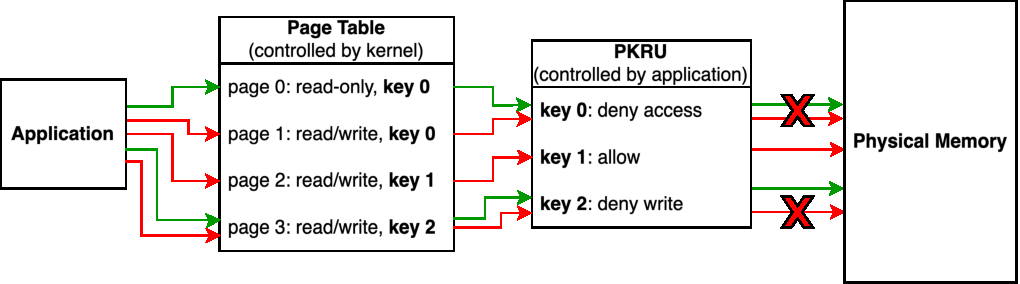
\includegraphics[width=\textwidth]{fig/mpk}
    \caption[Diagram of Memory Protection Keys]{Diagram of Memory Protection Keys. The kernel tags
    page table entries with a key (configurable with the \cc{pkey_mprotect} syscall). The user
    process can then restrict access to groups of pages by changing the permissions bits
    corresponding to a key in the PKRU register.}
    \label{f:mpk}
\end{figure}

This scheme allows a user program to manage its own sandbox: it can restrict or unrestrict regions
of memory at any time with a single register write -- without requiring expensive system calls,
context switches, or TLB flushes. It can't defend against all possible attacks: an attacker who can
take over the program's control flow may be able to use techniques such as return-oriented
programming to execute a \cc{wrpkru} instruction in order to disable the sandboxing and corrupt
protected memory. However, for our purposes of interoperability between memory-safe and
memory-unsafe code, it provides a low-overhead way to isolate the two and an effective line of
defense against memory corruption.

\paragraph{Prior Research} Prior research involving sandboxing using Memory Protection Keys includes
libmpk \cite{park:libmpk}, ERIM~\cite{vahldiek-oberwagner:erim}, Hodor~\cite{hedayati:hodor},
Cerberus~\cite{voulimeneas:cerberus}, Enclosure~\cite{ghoshn:enclosure} and
PKRU-safe~\cite{kirth:pkru}. libmpk by Park et al.~\cite{park:libmpk} implements a general-purpose
API that applications can use to manage protection keys, including a protection key virtualization
mechanism that applications can use to overcome the hardware limit of 16 protection keys; however,
it requires application developers to manually manage the keys and permissions associated with each
page of memory and configure the PKRU register appropriately before calling potentially unsafe
functions. ERIM by Vahldiek-Oberwagner et al.~\cite{vahldiek-oberwagner:erim} and Hodor by Hedayati
et al.~\cite{hedayati:hodor} explore the idea of software fault isolation with MPK, demonstrating
how this sandboxing can be used to protect applications in practice and implementing binary writing
techniques to prevent attackers from using control-flow hijacking to execute a \cc{wrpkru}
instruction and defeat the sandbox. Cerberus by Voulimeneas et al.~\cite{voulimeneas:cerberus}
extends this work further to defend against the possibility of unsafe code executing
attacker-controlled syscalls.

\paragraph{Automated Sandboxing} Enclosure by Ghoshn et al.~\cite{ghoshn:enclosure} automates the
process of creating sandboxed programs by extending mainstream programming languages with syntax to
manage sandboxing. PKRU-safe~\cite{kirth:pkru} by Kirth et al. directly addresses the problem of
sandboxing memory-unsafe code in memory-safe languages, and they do so using compiler extensions and
runtime instrumentation to perform provenance analysis of the program to determine what data
memory-unsafe code should have access to. Our work addresses the same problem as Kirth et al. --
sandboxing memory-unsafe code within memory-safe programs -- but our approach is implemented using
Rust's type system and procedural macros rather than requiring compiler or programming language
extensions.

\section{Other types of sandboxing} Sandboxing techniques can also be used to protect resources
other than memory, including filesystem, process, and networking resources. Linux provides
interfaces such as chroot~\cite {gnu:chroot}, seccomp/BPF~\cite {kim:mbox}, and Landlock~\cite
{linux:landlock} that can be used for this purpose. While our work limits the ability of sandboxed
code to take over its host program via memory corruption, it does not prevent sandboxed code from
compromising the system by e.g. writing to files or spawning a shell process; our work must be
combined with system call sandboxing techniques to prevent these attack vectors.

\chapter{Overview}

Our goal is to enforce low-overhead isolation through memory protection between memory-safe and
memory-unsafe code within a single process, in order to prevent memory corruption vulnerabilities
within memory-unsafe code from violating the integrity of the rest of the application. For example,
this type of sandbox may be used to protect an application from being compromised through a legacy
or 3rd-party library that parses attacker-controlled input and is written in a memory-unsafe
language. Consider a messaging application that uses a vulnerable image decoding library, which an
attacker can exploit by sending a malformed image to the victim: with proper fault isolation, the
attacker may be able to corrupt the decoded image data produced by the library, but they should not
be able to modify unrelated portions of the application's memory, such as the user's contacts or
message history (since that memory should not be accessed when decoding images). This is addressed
effectively by many existing MPK-based sandboxing schemes~\cite{vahldiek-oberwagner:erim,
hedayati:hodor, voulimeneas:cerberus, ghoshn:enclosure}.

Even if memory-unsafe code is protected from writing to protected regions of memory, an attacker may
still be able to indirectly cause corruption of protected memory by exploiting issues on the
boundary between memory-safe and memory-unsafe code. Application developers may misuse complex
sandboxing APIs and fail to correctly restrict memory access permissions when crossing boundaries
between protection domains. This is addressed by automatic sandboxing schemes such as PKRU-safe
\cite{kirth:pkru}, but even the current state-of-the-art schemes cannot enforce that safe code
properly validates sensitive values that are received from unsafe code. For instance, memory-safe
code may dereference an invalid pointer that was received from memory-unsafe code, causing undefined
behavior or memory corruption within memory-safe code that has write access to protected regions of
memory. Thus, we wish to develop a sandboxing scheme that provides a straightforward, safe API to
prevent misuse of the sandbox and improper validation of data exchanged across protection domains.

\section{Security Model}

We assume a program's code is divided into two portions: a "safe" portion written in Rust, and a
"sandboxed" portion written in C or C++. The two portions interact through function calls:
specifically, the safe portion can call functions defined in the sandbox portion. The two portions
can exchange data through function parameters and return values, and by reading and writing data
through pointers returned by these function calls (\autoref{f:sandbox}). Within the scope of our
work, we did not allow calls made in the other direction (C/C++ code calling functions defined in
Rust); additionally, we assume a single-threaded environment.

\begin{figure}[!ht]
    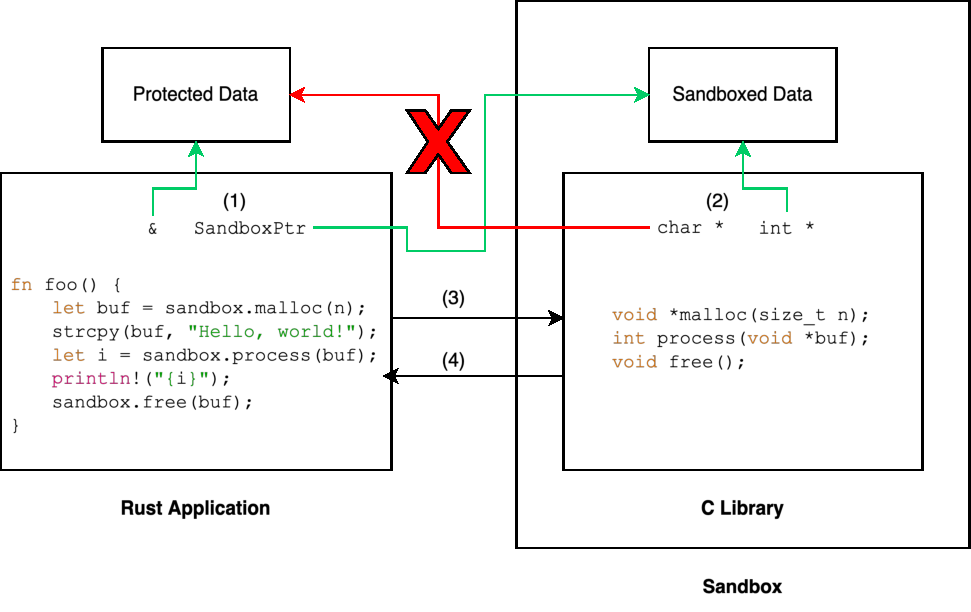
\includegraphics[width=\textwidth]{fig/sandbox}
    \caption[Diagram of our sandbox architecture]{Diagram of our sandbox architecture. Safe Rust
    code is allowed to access its own data (through Rust references) and sandboxed data (through a
    \cc{SandboxPtr} safe pointer type) (1). Unsafe C code can access sandboxed data, but is
    prevented from accessing memory belonging to the safe portion of the program (2). The safe Rust
    code can freely call functions defined in the unsafe portion of the program (3), and the two
    portions can exchange data through parameters and return values (4).}
    \label{f:sandbox}
\end{figure}

We assume the safe portion of our program is free from memory corruption; i.e., that there are no
implementation problems that would cause memory corruption within safe Rust code, and that any
\cc{unsafe} blocks within the Rust code are correctly written and cannot cause undefined behavior.
However, the "sandboxed" portion of our program is expected to contain memory corruption errors
(such as buffer overflows, uninitialized pointers, or use-after-free errors) that an adversary may
be able to exploit with the intent of corrupting variables used by the safe portion of our program.

We wish to define a security model that captures the intuitive idea that an attacker that exploits a
memory corruption vulnerability within sandboxed code can only corrupt memory intended to be
accessed by sandboxed code. This model is not intended to provide absolute security against all possible
memory-corruption attacks, but only on compartmentalization and fault isolation, to mitigate the
access an attacker has to a system after a successful exploit. Additionally, we only consider the
integrity of the application; our definition does not consider attacks on confidentiality (such as
exfiltrating sensitive information from the protected portion of the application) or availability (such
as crashing the application).

We formalize our intuitive model with \autoref{d:isolation}.

\begin{center}
    \centering
    \fbox{\parbox{\textwidth}{
        The sandboxed portion of a program is \textit{isolated} from the secure portion if the
        following conditions hold:
        \squishlist
            \item Memory allocated within safe code cannot be written by sandboxed code.
            \item Memory corruption caused by sandboxed code cannot induce undefined behavior within
                safe code.
        \squishend
    }}
    \captionof{definition}{Isolation}
    \label{d:isolation}
\end{center}

The first condition ensures that a bug in sandboxed code cannot corrupt memory used by unrelated
parts of the program; the second condition ensures that sandboxed code cannot behave in a manner
that could cause safe code to corrupt memory or otherwise behave unexpectedly -- for example, by
returning invalid pointers or values that violate ABI requirements such as alignment or aliasing
guarantees.

This definition is similar to the Biba integrity model~\cite{biba:integrity}. Biba's model asserts
that untrusted code should not be able to write to data owned by trusted code, that trusted code
should not read data owned by untrusted code, and that untrusted code cannot invoke functions
defined in trusted code. Our definition relaxes this second condition: trusted code is allowed to
read untrusted data as long as we can prove that the data is accessed in a manner which cannot cause
memory corruption or other undefined behavior.

Note that our sandbox only considers memory corruption that "escapes" the sandbox. Our work does not
aim to defend against memory corruption that only affects data accessed only within the sandbox, and
it does not aim to defend against attacks that escape the sandbox using means other than memory
corruption -- for example, system calls. An attacker that exploit memory corruption within the
sandbox to make arbitrary system calls could compromise the application without breaking our sandbox
as defined above; thus, to fully secure an application, our memory sandboxing technique must be
combined with a system call sandboxing technique such as mbox \cite{kim:mbox} or Landlock
\cite{linux:landlock}. For the remainder of our paper, we will consider attacks involving
attacker-controlled system calls to be out of scope, even if the attacker is able to gain control
over system calls through memory corruption.

\section{Deny Access or Deny Write?}

One design decision we faced was whether sandboxed code should be permitted read-only access to
protected data, or if protected data should be completely inaccessible. Allowing read-only access
could, in some cases, allow developers to avoid copying data from protected memory into the sandbox,
but it comes at a security disadvantage as sandboxed code could potentially exfiltrate sensitive
information from protected areas of memory.

We decided to choose a security model that only focuses on integrity: \textit{writing} to protected
memory within sandboxed code violates isolation, but reads are allowed. This decision was made to
simplify the implementation: the sandboxed code needs read access to the application memory image
and global offset tables in order to function, so creating a sandbox that protects against write
access would require special-case handling of this memory. (It is not a limitation of our approach;
a straightforward extension of our work would be to use separate protection key to permit read-only
access to non-sensitive data located within the program binary image while denying reads from
sensitive data in the program's data section or heap.) A security model that prevents sandboxed code
from reading from protected memory would contain conditions resembling the Bell-LaPadula
model~\cite{bell:confidentiality}, which describes data confidentiality rather than integrity.
Complete isolation ensuring both confidentiality \textit{and} integrity under both the Biba and
Bell-LaPadula models would prevent interoperability between the safe and sandboxed code entirely (as
the two regions would not be allowed to communicate at all); therefore, we chose to implement a
relaxed Biba integrity model in order to achieve a useful definition of security that allows for a
functional system. 

\section{Enforcing Isolation with Sandboxing}

While the above definitions have made a distinction between sandboxed and safe \textit{code}, we
implement our sandbox by distinguishing between sandboxed and safe \textit{data}. Specifically, we
define all data that is intended to be accessed by sandboxed code as sandboxed data; and all data
that is intended to be accessed solely by safe code as safe data. At every function call into
sandboxed code or returning from such a function, we use the \cc{wrpkru} instruction to restrict or
unrestrict access to safe data accordingly. This instruction modifies the MPK registers to quickly
enable or disable access to regions of memory entirely within userspace, achieving much better
performance than schemes that require invoking the kernel (such as process switching or system calls
such as \cc{mprotect}).

In practice, sandboxed code needs access to any global or static variables defined within that
sandboxed code, but it should not have access to globals defined within safe code. Sandboxed code
needs access to any heap memory that it allocated, but it should not have access to heap memory
allocated by safe Rust code. And sandboxed code needs access to its own stack memory for return
addresses and local variables, but it should not be able to access return addresses and local
variables of safe code.

To achieve this, our work uses memory protection keys to partition the program's address space into
two regions: the "sandboxed" region, which is always accessible by any part of the program, and the
"protected" region, which is accessible to safe code but inaccessible to sandboxed code.

\section{Type-Safely Preventing Undefined Behavior with bindgen}

While the use of memory protection keys as described above is sufficient to achieve the first
condition necessary for isolation, it does not achieve the second. Sandboxed code may return or
write to output parameters values that are illegal under the platform's application binary interface
(ABI), and this induces undefined behavior in safe code that tries to access those values. For
instance:

\squishlist
    \item Sandboxed code may return values that are invalid for the given type -- for example,
        returning a value of boolean type that is neither 0 nor 1.
    \item Sandboxed code may fail to uphold alignment guarantees.
    \item Sandboxed code may return pointers that are null, misaligned, invalid, or point to safe
        memory.
    \item Sandboxed code may return pointers that violate Rust's aliasing and single-mutability
        rules.
\squishend

Rust's \cc{bindgen} "solves" this by marking all generated bindings as \cc{unsafe}: indicating
that invoking them may invoke undefined behavior, and that it is the programmer's responsibility to
verify all relevant memory safety invariants are upheld. Additionally, pointers used as arguments or
return values to C functions are imported to Rust as raw unsafe pointers rather than safe
references; again indicating it is the programmer's responsibility to uphold memory safety when
working with raw pointers.

This is the simplest and most straightforward way of binding to C libraries from Rust programs, and
the semantics are reasonable: when calling into C code, programmers get C's safety guarantees (or
lack thereof). However, we did not consider this an acceptable level of safety for our project. The
complexity of this boundary and the number of invariants it places on the programmer create a high
attack surface, which an attacker with memory corruption within the sandboxed portion of the program
can exploit to induce undefined behavior in the safe portions and pivot to memory corruption there
as well.

Therefore, we modified \cc{bindgen} to provide stronger guarantees in our context of calling into
a sandboxed C library from a Rust program. Notably, we are able to use Rust's type system to express
the requirements and invariants around working with a sandbox, such that we do not need to mark
bindings to sandboxed functions as \cc{unsafe}, and applications can use Rust's safe reference
types to interact with sandboxed data rather than using unsafe raw pointers. Our implementation
transforms all pointer types in C function signatures to safe Rust wrapper types that verify
invariants such as pointer bounds and alignment, and enforce the aliasing requirements needed to
safely interact with sandboxed data using Rust reference types.

\chapter{Design}
\section{Enforcing Isolation with Memory Protection Keys}

In order to maintain separation between sandboxed and protected data, we assign the default memory
protection key (with ID 0) to the executable image, the data section associated with Rust code, all
heap pages allocated by Rust code, and the Rust stack. (We use the default key for this purpose so
that we don't need to make extensive changes to the Rust build process and runtime libraries --
everything that we don't explicitly assign a protection key uses the default key.) We allocate a
second protection key for sandboxed data, and we assign this key to the data section of all C object
files, all heap pages allocated by sandboxed code, and a dedicated stack we allocate for sandboxed
code.

We define a thunk function that handles calls from safe functions to a sandboxed function. This
function:

\squishlist
    \item Copies the function parameters onto the sandboxed stack.
    \item Saves the safe stack pointer to a static variable living within protected memory at a constant
        address (relative to the program image base under address-space layout randomization).
    \item Switches the \cc{rsp} register to point to the sandboxed stack.
    \item Uses the \cc{wrpkru} instruction to disable read access to safe memory.
    \item Calls the sandboxed function using the parameters saved to the sandboxed stack, saving the
        return value to the sandboxed stack.
    \item Uses the \cc{wrpkru} instruction to re-enable write access to safe memory.
    \item Restores the safe stack pointer.
    \item Returns to the safe caller, passing the return value obtained from the sandboxed stack.
\squishend

\bigskip
As long as all calls to sandboxed functions go through this thunk function, our implementation
enforces the first condition of isolation as defined above (but not the second, yet). The use of
memory protection keys enforce that any attempt by the sandboxed code to corrupt safe memory will
cause an access violation, and the use of a separate stack for sandboxed code is necessary to
prevent stack buffer overflows and similar forms of memory corruption from affecting local variables
and return addresses use by safe code. It is important that the safe stack pointer be stored in a
location that is protected from writes by MPK so that an attacker who exploits bugs in sandboxed
code cannot point the safe stack somewhere else; the fact that the stack pointer is restored
immediately after the $\cc{wrpkru}$ instruction also prevents an attacker from hijacking the
program's control flow after returning from a sandboxed function call.

\begin{figure}[!ht]
    \centering
    \includegraphics{fig/stack}
    \caption[Diagram of stack usage]{Diagram of stack usage. Sandboxed code is on a separate stack
    so it cannot corrupt local variables and return addresses belonging to safe code. The
    \cc{RETURNSTACK} global variable tracks the original location of the stack pointer when
    returning from sandboxed code. MPK is used to enforce that sandboxed code cannot write to the
    protected stack or the \cc{RETURNSTACK} pointer.}
    \label{f:stack}
\end{figure}


There is one caveat with the implementation as described above: if an attacker can cause sandboxed
code to execute the \cc{wrpkru} instruction, they may be able to remove the protections on safe
memory and then proceed to violate isolation. To prevent this attack vector, we require that the
program must never execute the \cc{wrpkru} instruction except in the teardown portion of the thunk
function. This means that the instruction should never be intentionally executed by the program
outside of the thunk function, and that an attacker should not be able to use control-flow hijacking
techniques such as Return-Oriented Programming to cause the execution of a \cc{wrpkru} instruction.
Thus, we require the program use some form of control flow protection such as x86 Control-flow
Enforcement Technology (CET) to prevent an attacker from being able to reach a \cc{wprkru} gadget,
or binary rewriting techniques such as those employed by Vahldiek-Oberwagner et
al.~\cite{vahldiek-oberwagner:erim} or Hedayati et al.~\cite{hedayati:hodor} to prevent the compiler
from generating executable byte sequences that could be interpreted \cc{wrpkru} instructions.

\section{Type-Safely Preventing Undefined Behavior with bindgen}

Our modified version of \cc{bindgen} applies the following modifications to the generated Rust bindings to C code:

\squishlist
    \item Functions are imported as member functions on a "sandbox object", rather than free
        functions. (The sandbox object uniquely identifies a sandbox domain with an associated
        memory protection key and sandbox stack).
    \item Functions are wrapped using the thunk described in the previous section, which sets up the
        sandbox permissions appropriately before dispatching to the sandboxed code.
    \item All types involved in function parameter or return types must conform to
        \cc{AnyBitPattern}, a marker trait provided by the \cc{bytemuck} crate denoting types
        with no invalid representations.
    \item All pointer types are converted to wrapper types named \cc{SandboxPtr} (for \cc{const}
        pointers) and \cc{SandboxPtrMut} (for mutable pointers), which verify at runtime that the
        pointers are valid and point to sandboxed data, and allow for safe Rust access to the
        pointer contents.
\squishend

For example, a C function with signature \cc{const int *foo(int *p)} maps to the Rust binding shown
in \autoref{c:binding-example}. The generated assembly is shown in \autoref{c:binding-example-asm}.

\begin{figure}[ht]
\input{code/binding-example.rs}
\coderule
\caption[Example of generated Rust bindings to a C function]{
    Example of bindings generated from a C function with signature \cc{const int *foo(int *p)}.
    The underlying C function is imported privately (in the \cc{extern "C"} block), and a publicly
    accessible wrapper function is generated which uses our runtime library to move parameters into
    sandboxed memory, update the PKRU to restrict access to protected memory, call the sandboxed
    function, restore the previous value of the PKRU, and validate the returned pointer.
}
\label{c:binding-example}
\end{figure}


\begin{figure}[ht]
\input{code/binding-example.asm}
\coderule
\caption[Example of generated Rust bindings to a C function, compiled output]{Example of generated
    bindings, compiled output (error-handling slow-path code omitted for brevity). The generated
    assembly initializes MPK if it has not been done yet, switches the stack pointer to the
    sandboxed stack, updates the PKRU, calls the sandboxed function, and restores the old PKRU and
    stack pointer before returning.}
\label{c:binding-example-asm}
\end{figure}

\section{Safe Pointers to Sandboxed Data}
\label{s:aliasing}

Safe Rust code is not allowed to use raw pointers directly, because use of raw pointers requires the
programmer to uphold a set of invariants that are not checked by the compiler:

\squishlist
    \item If a pointer is accessed, it must be non-null, properly aligned,
        and point to a valid object of the correct type.
    \item If a pointer is converted to a safe reference type, we must uphold the aliasing rules.
    \squishlist
        \item If a mutable reference exists to an object in memory, that reference must be unique
            throughout its entire lifetime (i.e. no other reference to the same object may exist for
            as long as the mutable reference is valid)
        \item If an immutable reference exists to an object in memory, that object must not be modified.
        \item If a mutable reference exists to an object in memory, that object must not be accessed
            at all except via the mutable reference.
    \squishend
\squishend

In order to allow Rust code to safely interact with sandboxed memory, we allow a \cc{SandboxPtr}
or \cc{SandboxPtrMut} to be converted into a safe Rust reference. We use the type system to ensure
that all of these invariants are upheld:

\squishlist
    \item The constructor for a \cc{SandboxPtr} or \cc{SandboxPtrMut} verifies the pointer's
        alignment, and checks that the pointer points to an object contained within the bounds of
        the sandbox. This check ensures that sandboxed code that is buggy or compromised cannot
        return a pointer to protected data, which could cause our Rust program to corrupt memory or
        violate aliasing rules. Additionally, conversion to a reference includes a null check.
    \item Converting a \cc{SandboxPtr} or \cc{SandboxPtrMut} to a reference requires the caller
        to have a reference of matching mutability and lifetime to the sandbox object (and calling a
        sandboxed function requires a mutable reference to the sandbox object). This enforces the
        aliasing rules:
    \squishlist
        \item Since creating a mutable reference requires a mutable reference to the sandbox object,
            only one mutable reference to sandboxed data may exist at a time. This ensures that the
            single-mutability rule is not violated even if sandboxed code returns unexpectedly
            overlapping pointers.
        \item Since creating an immutable reference requires an immutable reference to the sandbox
            object, no mutable references to sandbox data may be created  while an immutable
            reference exists. However, the programmer may freely create multiple immutable
            references to sandboxed data.
        \item Since calling a sandboxed function requires a mutable reference to the sandbox object,
            sandboxed functions may not be called (and thus cannot modify memory) while references
            to sandboxed memory exist.
    \squishend
\squishend

Our approach allows programs to freely interact with C APIs that consume and return pointers to
objects in memory, without requiring the use of \cc{unsafe} blocks and without risk of undefined
behavior. The limitation that only one mutable reference to sandboxed data can exist at any time is
a severe restriction to our model, but some form of this restriction must exist in order to ensure
the aliasing rules are upheld in the presence of misbehaving code inside the sandbox. If needed,
programmers can circumvent these restrictions with the use of an \cc{unsafe} block, and our work
can be extended to relax these restrictions somewhat (for example, by checking for aliasing at
runtime).

\chapter{Implementation}

Our implementation consists of a 270-SLOC Rust library containing type definitions and runtime code
to implementing memory protection, and a 170-line patch to \cc{bindgen} to generate thunk functions
for imported C libraries.

We define a trait \cc{SandboxSafe} that represents types that are safe for Rust code to access, even
when its contents may be untrusted. For example, an integral type is \cc{SandboxSafe} because no
values of an integer can cause undefined behavior; a boolean type is \textit{not} \cc{SandboxSafe}
because there are many possible byte values that result in invalid values when interpreted as a
boolean type. We automatically implement this trait for types implementing the \cc{AnyBitPattern}
trait defined in the \cc{bytemuck} crate~\cite{bytemuck:AnyBitPattern}.

We define types \cc{SandboxPtr} and \cc{SandboxPtrMut} that provide wrappers around unsafe pointers
that point into sandboxed data. The constructors for these types check to ensure the pointers are
valid, properly aligned, and point within the sandbox. If the pointee type implements
\cc{SandboxSafe}, we provide functions allowing the user to obtain a safe Rust reference or slice to
the referenced data.

We define a \cc{Sandbox} object representing a protection domain. The sandbox defines the \cc{call}
method, which requires a unique reference to the sandbox object (to enforce the aliasing constraints
discussed in \autoref{s:aliasing}), and takes in a closure which is run with the permission
restrictions of the sandbox. Closures in Rust can carry captured state, which the \cc{call} moves
onto the dedicated sandbox stack, allowing the user to pass arbitrary data such as function
parameters into the sandbox. The sandbox stack is also used to store the return value of the
provided closure, which is copied back to the caller.

\section{Sandboxed code and libc}

We did not address the problem of linking sandboxed code to the C standard library. The reason for
this is that Rust code also links to and relies on the standard library. This would cause internal
libc data structures to be shared by both sandboxed and safe code. We cannot mark memory used by
libc as sandboxed because then sandboxed code could trivially corrupt memory that is used when Rust
code calls libc functions, violating our first condition of isolation in \autoref{d:isolation}. We
also cannot mark memory used by libc as protected because libc functions would then need to be
trusted in order for them to access libc memory, and sandboxed code could pass invalid pointers into
libc functions to cause undefined behavior in trusted code, violating the second condition of
isolation.

One solution to this problem would involve two independent copies of libc; a trusted libc used by
safe code and a sandboxed libc used by sandboxed code. The two copies would not share internal state
and thus not suffer from the problems described above. We attempted implementing this with two libc
implementations: nolibc (a minimal, header-only libc implementation included with the Linux
kernel)~\cite{lwn:nolibc} and musl~\cite{musl}. Both of these attempts were unsuccessful: nolibc
depended on header files and build tooling from the Linux kernel, and was nontrivial to build
outside of that environment; whereas musl would not easily coexist in the same process as glibc.
Next steps for future work on this problem could include modifying a libc implementation to support
secure interaction with both trusted and untrusted code in the same process, and/or identifying or
creating a libc implementation that supports multiple separate instances of libc in the same
process.

\chapter{Evaluation}
\label{s:eval}

\paragraph{Evaluation Goals} We evaluated our work on security and performance. We want our work to
meet the conditions established in \autoref{d:isolation}, and we want performance overhead to be
within acceptable levels. When we designed our approach, our target for performance was a negligible
slowdown within both memory-safe code and memory-unsafe code, with only a small performance penalty
when entering or exiting a sandboxed function.

\section{Security}

Recall our security definition in \autoref{d:isolation}. In order for our sandboxing scheme to be
considered secure, the sandboxed portion of the program must not allow sandboxed code to write to
memory allocated within safe code, and it must prevent memory corruption that occurs within
sandboxed code from causing undefined behavior within safe code.

We use MPK to enforce our first condition ("Memory allocated within safe code cannot be written by
sandboxed code"). In particular, we achieve this by our configuration of the PKRU register to deny
write access to protected data upon entering sandboxed code, and to re-enable write access upon
exiting sandboxed code. More specifically, we assume the processor's implementation of MPK is itself
correct and secure (in other words, that an attacker truly cannot write to memory restricted by
MPK).

We also must ensure that an attacker with partial or complete control over the program's execution
cannot cause a \cc{wrpkru} instruction to be executed and maintain control of the program
afterwards, as this would potentially allow an attacker to disable the sandboxing restrictions and
corrupt protected memory. We enforce this by ensuring the return address and call stack used by safe
code are not writable by sandboxed code, preventing the attacker from using a backward-edge control
flow hijacking attack to redirect code execution after the program returns from the sandbox to safe
code. Additionally, we require that the program does not use the \cc{wrpkru} instruction except for
entering and exiting the sandbox, and we require the use of Control-flow Enforcement Technology
(CET) to prevent the attacker from using a forward- or backward-edge control flow hijacking attack
(such as function pointer hijacking or return-oriented programming) to cause the execution of a
\cc{wrpkru} instruction.

The second condition is more difficult to verify, as in general, it is impossible to reason about a
program in the presence of undefined behavior such as memory corruption. In theory, the compiler
could identify undefined behavior in the sandboxed code and as a result generate \cc{wrpkru}
instructions that defeat our sandboxing; generate unexpected code within the safe portions of our
program that assume the sandboxed portions do not induce undefined behavior; trigger unknown
processor bugs that defeat MPK, or ``make demons fly out of your nose'' (as the saying goes).
However, in order to reason about systems security, we must make assumptions constraining undefined
behavior to reasonable limits. Since an attacker can and will exploit undefined behavior to attack a
system, we must design our systems to maintain their security model in the presence of undefined
behavior, and we must rely on the layers below us to uphold the security guarantees we rely on. For
instance, operating systems must assume that a processor's memory protection guarantees apply even
in the presence of a program inducing undefined behavior; system call interfaces must uphold their
security models even when provided with invalid or impossible inputs; and in-process sandboxing
schemes like ours must assume the compiler does not introduce optimizations that violate our
sandboxing requirements even in the presence of undefined behavior. In practice, this assumption may
not always hold; designing systems that are correct in the face of unexpected compiler behavior is a
limitation of any in-process sandboxing scheme and an area of active research.

Proceeding under the assumption that undefined behavior within the sandbox does not somehow disable
the sandbox, then to verify the second condition we only need to consider how the safe portions of
our program react upon receiving untrusted outputs from the sandbox. The Rust language guarantees no
undefined behavior, as long as the safe portions of our program do not incorrectly use \cc{unsafe}
language features, and as long as any \cc{unsafe} blocks do not return invalid values to the safe
portions of the program. Our \cc{bindgen}-generated interface contains \cc{unsafe} blocks for
integrating with unsafe code, but we believe all our \cc{unsafe} code to be correctly written and
free of undefined behavior. Our requirement that types exchanged across sandbox boundaries conform
to \cc{bytemuck::AnyBitPattern} means that unsafe code cannot produce invalid values (as no such
invalid values exist), and our bounds, alignment, and aliasing checks on pointers exchanged across
sandboxed boundaries ensures that invalid pointers cannot cause undefined behavior.

There may be a risk of induced undefined behavior through application binary interface (ABI)
violations. For instance, calling conventions typically specify a set of registers that are expected
to be preserved across function calls; most x86 calling conventions require that the direction flag
be clear when calling and returning from functions; and the ARM procedure call standard requires
that signed types shorter than 32 bits be sign extended when passed in registers. In theory, a
sandboxed application may induce undefined behavior in the safe portions of the program by violating
these ABI constraints; while our proof-of-concept is potentially vulnerable to this attack vector,
our work can be extended to defend against this possible attack by modifying the sandbox thunk
function to carefully verify ABI invariants upon exiting sandboxed code.

\section{Performance}

Our implementation only affects code generation when memory-safe code calls and returns from a
function defined in a sandboxed library. The sandboxed library remains unchanged, as does most of
the Rust application (aside from potential application-specific needs to copy data into or out of
sandboxed memory). Thus, we expect the performance impact of our work to manifest as a fixed
overhead per function call into a sandboxed library. Applications that interact with sandbox
libraries frequently via many short-lived function calls are expected to suffer the greatest
performance overhead, whereas we expect the performance impact to be negligible for applications
that make few or longer-running function calls.

To test this, we used the \cc{cargo bench} tool available in nightly Rust \cite{rust:cargo-bench}.
We created a series of three benchmarks: a microbenchmark which calls a sandboxed no-operation
function (to measure the overhead of a single function call), a second test case which uses the
\cc{cmark} Markdown parsing library \cite{cmark} to render a short string of Markdown into HTML, and
a third which uses \cc{cmark} to render a long document (created by concatenating all localizations
of the first edition of Pro Git \cite{pro-git}, as this is the document used by the authors of cmark
in their own benchmarks \cite{cmark:benchmarks}). \cc{cargo bench} automatically runs a sufficient
number of iterations of each benchmark to ensure statistically significant results, with the
iteration count determined dynamically based on the runtime of each tests and the level of noise in
the results. The \cc{nop} and \cc{cmark\_simple} microbenchmark results reported are an average over
several million iterations, and the \cc{cmark\_large} benchmark is an average over several hundred
iterations. We ran our benchmarks on an Intel NUC with an i5-1135G7 CPU running at 2.4 GHz.

We ran each test case under three conditions: once with sandboxing and control-flow enforcement
disabled to establish a baseline; once with sandboxing disabled but CET enabled so that we can
determine how much performance impact is caused by our sandbox and how much is caused by CET; and a
third time with sandboxing and CET enabled. The results are available in \autoref{bench-txt},
\autoref{f:graph1}, and \autoref{f:graph2}. \cc{cargo bench} is designed for accurate
microbenchmarking and runs each test case a sufficient number of iterations to obtain statistically
meaningful results.

\begin{figure}[ht]

\begin{subfigure}{1\textwidth}
\input{code/bench-nocet.txt}
\coderule
\caption{Sandboxing and CET disabled}
\end{subfigure}

\begin{subfigure}{1\textwidth}
\input{code/bench-nompk.txt}
\coderule
\caption{Sandboxing disabled, CET enabled}
\end{subfigure}

\begin{subfigure}{1\textwidth}
\input{code/bench-mpk.txt}
\coderule
\caption{Sandboxing and CET enabled}
\end{subfigure}

\caption{Benchmark results}
\label{bench-txt}
\end{figure}

\begin{figure}[ht]
    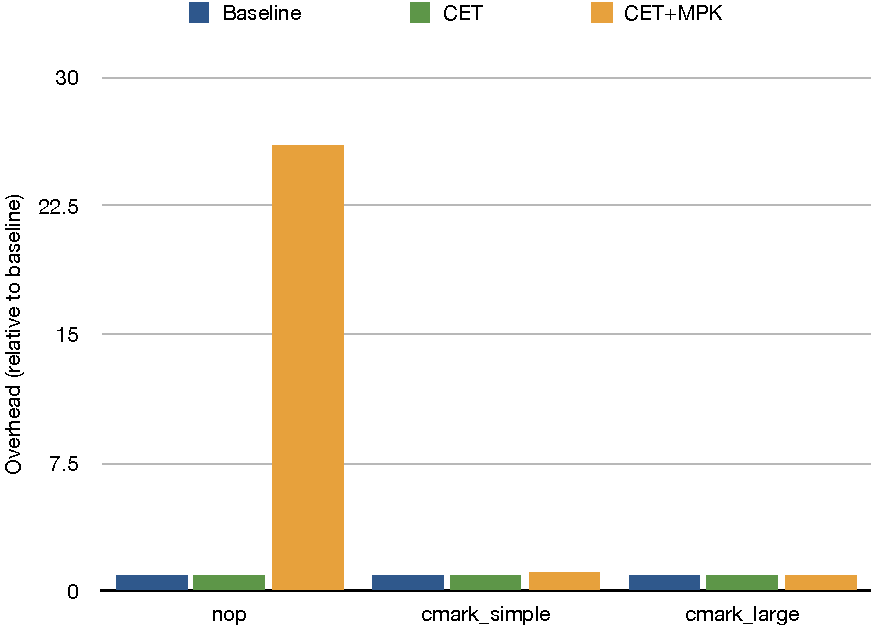
\includegraphics[width=\textwidth]{fig/graph1}
    \caption{Graph of benchmark results.}
    \label{f:graph1}
\end{figure}

\begin{figure}[ht]
    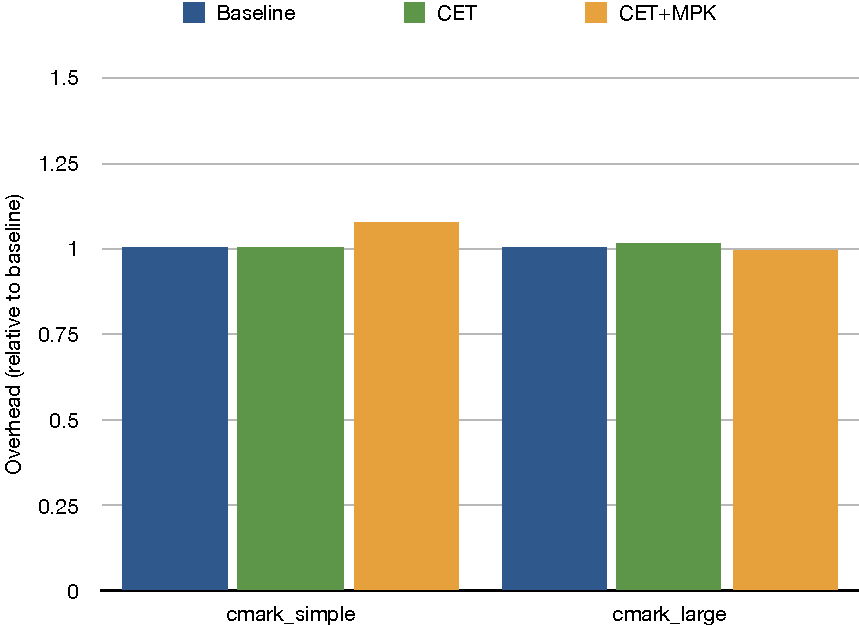
\includegraphics[width=\textwidth]{fig/graph2}
    \caption{Graph of benchmark results, excluding the \cc{nop} benchmark.}
    \label{f:graph2}
\end{figure}

The no-operation benchmark shows an overhead of approximately 25 nanoseconds due to our sandbox for
a single function call, compared to a baseline of 1ns. The small cmark benchmark runs approximately
50 nanoseconds slower when sandboxing is enabled, an overhead of about 7\%; this is consistent with
the no-op test case as the small cmark test case makes two sandboxed function calls. For the
longer-running cmark test case, the performance impact is not statistically significant (as the work
required to enter and exit the sandbox is dwarfed by the work performed within the sandbox.) The
benchmark results show no statistically significant performance impact caused by the use of CET. 

\chapter{Discussion}

\section{Limitations and future direction}

We only address the issue of memory corruption; other types of security vulnerabilities that can be
caused by unsafe or untrusted code are outside the scope of our research. Additionally, we do not
aim to \textit{prevent} memory corruption within untrusted code, only to isolate the untrusted code
to limit the capabilities of memory-corruption based attacks. Our security model does not prevent an
attacker from using memory corruption to change the output of sandboxed code, or even achieving full
remote code execution with the limitation of only being able to write to memory used by the
sandboxed portions of the program.

Notably, we do not consider the effects of system calls. An attacker could corrupt memory within the
sandboxed portion of a program and cause the program to execute system calls that (for instance) run
arbitrary shell commands, corrupt memory indirectly using operating features like the \cc{/proc}
filesystem, or disable memory protection features with \cc{mprotect} or related syscalls. Thus,
our sandboxing scheme must be combined with a system call sandboxing scheme to achieve security
against such attacks.

Our implementation does not properly support dynamically linking to sandboxed libraries, or calling
dynamically-linked functions from within a sandbox. This is not a fundamental limitation of our
technique, but rather a feature that is unsupported by our proof-of-concept research implementation.
Dynamic linking should be relatively straightforward to support, as dynamically linked libraries are
loaded as separate images in memory with separate global offset tables, data sections, etc., making
it easier to identify the boundaries of the sandbox than for static libraries.

Additionally, our work supports calls from safe code into unsafe code, but we have not explored the
other direction: unsafe code calling functions written in a safe language. Extending our techniques
to support calls in both directions is a useful future direction for our research.

We only support running sandboxed code on a single thread, due to the aliasing requirements for
Rust's reference types: in order to verify that immutably-referenced data is not modified and that
mutably-referenced data is not aliased, we enforce through the type system that no sandboxed code
can be running while Rust code is interacting with its memory. Extending our approach to support
multithreading would require significant changes to this model.

\section{Other architectures}

Our implementation only functions on x86, because MPK is an x86-specific feature. Our approach could
be ported to other architectures, provided similar hardware or software functionality allowing for
sufficiently low-overhead memory protection domains that can be changed by the user application at
runtime.

\paragraph{RISC-V} Schrammel et al.~\cite{schrammel:donky} implement a hardware extension for RISC-V
allowing a page table entry to specify one of up to 1024 domain keys, in addition to the standard
page table permission bits. A user program can write to the \cc{DKRU} register to configure
permission restrictions on a per-key basis, similar to MPK on x86. Their approach supports up to
1024 domain keys, allowing for many more protection domains than MPK (which is limited to 16), but
only four domain keys can be active at any given time (memory protected by an inactive key is
inaccessible to the program).

\paragraph{Arm} The AArch32 architecture supports configurable domains in AArch32 with a similar
implementation to MPK, except that reconfiguration of memory domains is only available in privileged
mode; a user program using the feature for software fault isolation would thus need to issue a
system call whenever it needs to change memory permissions. The feature is primarily designed for
allowing faster context switches on embedded systems rather than application-level sandboxing, and
was removed in AArch64.

Apple maintains a proprietary extension for ARM known as SPRR~\cite{peter:sprr}. With this
extension, page table permission bits are repurposed as indices into a table that can be configured
using system registers, some of which are user-accessible. Apple currently uses this functionality
to enforce $\text W \oplus \text X$ permissions for programs using JIT-compiled code, exposing userspace APIs which
write to these system registers to quickly toggle regions of memory between writable and executable
without requiring a system call~\cite{apple:jit}. This functionality could be used (within a
modified macOS or Asahi Linux~\cite{asahi} kernel) to implement software fault isolation on devices
with Apple processors.

\chapter{Related Work}

In this section, we compare our work to other research in this area, namely Enclosure by Goshn et
al. \cite{ghoshn:enclosure} and PKRU-safe by Kirth et al. \cite{kirth:pkru}.

\paragraph{Enclosure} Ghoshn et al.~\cite{ghoshn:enclosure} implemented a language-level approach to
sandboxing, using either MPK or Intel VT-x to divide the memory space into \textit{enclosures} that
are accessible only by the owning module. Their work extends contemporary programming languages with
syntax and semantics to support the notion of calling functions defined in other enclosures and
exchanging data between enclosures. Their work is more generalized than ours, supporting many
enclosures in the same program, along with nested enclosures, and allowing precise specification
over how data should be shared between enclosures. However, they do not appear to address the issue
of misbehaving enclosed code inducing memory corruption within the calling code, such as by
returning invalid pointers.

\paragraph{PKRU-safe} Kirth et al.~\cite{kirth:pkru} address the same problem as us: isolating memory-safe Rust
programs from memory-unsafe dependencies. Their implementation functions without requiring any
modifications to the Rust application or each dependencies, by using dynamic instrumentation to
determine which of the program's heap allocations should be accessible from unsafe dependencies and
using the results of the instrumentation to apply memory protection keys.

This approach is both a strength and a weakness: functioning with zero code changes is a significant
advantage over our approach. However, it also requires significant compiler modifications whereas
our work functions on unmodified, upstream \cc{rustc}. Their use of dynamic program analysis to
determine the sandbox boundaries raises the possibility of the boundaries being placed in incorrect
or unexpected locations: if their instrumentation pass does not achieve full coverage of the
program, it may misidentify whether an allocation needs to be accessible from within sandboxed code,
causing crashes at runtime. Additionally, since the analysis happens implicitly and automatically,
PKRU-safe may decide that an allocation needs to be accessible from sandboxed code even though the
developer expects it to be protected. For these reasons, we decided on an approach that uses static
type-based analysis and requires the developer to explicitly consider and delineate sandbox
boundaries within their source code. Lastly, PKRU-safe does not protect stack variables or global
variables, and (like Enclosure) does not address the issue of unsafe code inducing memory corruption
by returning invalid values to safe code.

Both of these approaches have advantages and disadvantages as compared to our work. We believe our
work demonstrates that low-overhead, secure, and practical sandboxing can be to implement in
production software today with no need for custom tooling or new programming language features.
Additionally, we believe our approach of using the type system to allow safe code to freely access
pointers to sandboxed data is a novel approach to preventing undefined behavior and ensuring
security when exchanging data across a sandbox.

\chapter{Conclusion}

We demonstrate that MPK can be used to provide lightweight, low-overhead, and robust sandboxing of
memory-unsafe code within a Rust program. Our technique both prevents undefined behavior in
memory-unsafe code from corrupting memory used by safe portions of the program, and additionally
prevents invalid values (such as corrupt pointers) returned from memory-unsafe code from inducing
undefined behavior within memory-safe portions of the program. We implemented a modified version of
\cc{bindgen} to automatically generate thunk functions to securely and type-safely call and return
from sandboxed functions, with a performance overhead of approximately 25ns per function call
on our test system.


\bibliographystyle{plain}
\bibliography{thesis,conf}

\end{document}
